% --------------------------------------------------------------
% This is all preamble stuff that you don't have to worry about.
% Head down to where it says "Start here"
% --------------------------------------------------------------
 
\documentclass[12pt]{article}
 
\usepackage[margin=1in]{geometry} 
\usepackage{amsmath,amsthm,amssymb}
\usepackage[UTF8]{ctex}
\usepackage[colorlinks=true,citecolor=blue]{hyperref}%
\newcommand{\N}{\mathbb{N}}
\newcommand{\Z}{\mathbb{Z}}
 
\newenvironment{theorem}[2][Theorem]{\begin{trivlist}
\item[\hskip \labelsep {\bfseries #1}\hskip \labelsep {\bfseries #2.}]}{\end{trivlist}}
\newenvironment{lemma}[2][Lemma]{\begin{trivlist}
\item[\hskip \labelsep {\bfseries #1}\hskip \labelsep {\bfseries #2.}]}{\end{trivlist}}
\newenvironment{exercise}[2][Exercise]{\begin{trivlist}
\item[\hskip \labelsep {\bfseries #1}\hskip \labelsep {\bfseries #2.}]}{\end{trivlist}}
\newenvironment{reflection}[2][Reflection]{\begin{trivlist}
\item[\hskip \labelsep {\bfseries #1}\hskip \labelsep {\bfseries #2.}]}{\end{trivlist}}
\newenvironment{proposition}[2][Proposition]{\begin{trivlist}
\item[\hskip \labelsep {\bfseries #1}\hskip \labelsep {\bfseries #2.}]}{\end{trivlist}}
\newenvironment{corollary}[2][Corollary]{\begin{trivlist}
\item[\hskip \labelsep {\bfseries #1}\hskip \labelsep {\bfseries #2.}]}{\end{trivlist}}
 
 
 \usepackage[usenames, dvipsnames]{color}
 \usepackage{graphicx}
 
 \definecolor{mypink1}{rgb}{0.858, 0.188, 0.478}
 \definecolor{mypink2}{RGB}{219, 48, 122}
 \definecolor{mypink3}{cmyk}{0, 0.7808, 0.4429, 0.1412}
 \definecolor{mygray}{gray}{0.6}
 \definecolor{myblue}{RGB}{0,0,255}
 \definecolor{myblack}{RGB}{0,0,0}
 \definecolor{myChocolate}{rgb}{0.824, 0.412, 0.118}
 \definecolor{myOrange}{rgb}{1.000, 0.647, 0.000}
 
\begin{document}
 
% --------------------------------------------------------------
%                         Start here
% --------------------------------------------------------------
 
%\renewcommand{\qedsymbol}{\filledbox}
 
\title{光线追踪术语}%replace X with the appropriate number
\author{Eric Haines and Peter Shirley \\
	翻译:RainVector} 
 
\maketitle
\tableofcontents
 \section{光线追踪基础}
今天,光栅化主导了大多数应用领域的实时渲染,因此许多寻找实时渲染技巧的读者在学生时代(可能几十年前)就接触过光线追踪。本部分包含了各种介绍性的章节来帮助大家温习基础知识,建立一个通用的词汇表,并提供简单(却很有用)的基础模块。

章节\color{blue}1\color{black}, “光线追踪术语” 定义了整本书都要用到的一些通用的术语并且参考了引入这些术语的开创性研究论文。对于新手读者来说,当你深入研究文献时,会出现很多令人困惑、含义不断变化、各种重叠且命名不佳的术语。在不理解这些术语如何演化到今天使用的这样子,直接去读30年前的论文会是一个令人沮丧的过程。本章节提供了一个基础的路线图。

章节\color{blue}2\color{black},“什么是光线?”,覆盖了一些通用的光线的数学定义:如何看待光线,哪些公式通常会用于现代API中。 虽然这是一个简单的章节,但是从基础部分分离出这个基本结构会有助于提醒读者数值精度问题比比皆是。对于光栅化,z-fighting 和阴影映射(Shadow Mapping)会出现精度问题;在光线追踪中,每一次光线查询都需要小心处理以避免虚假交叉(精度问题在章节6会有更多的介绍)。

最近,微软公司推出了DirectX光线追踪技术,它是DirectX 光栅化API的扩展。章节\color{blue}3\color{black},\ “DirectX 光线追踪介绍”,简单介绍了这个编程接口引入的抽象,心智模型和新的着色器阶段。除此之外,还介绍并解释了初始化API所需的步骤,并提供了示例代码以帮助您入门。

光线追踪器允许我们很容易得构建任意一个相机模型,而不像传统的光栅化API那样定义一个$4\times 4$的投影矩阵来限制相机。章节\color{blue}4\color{black},“一个天文馆圆顶主摄像机”给出了构建一个180度半球形圆顶投影(比如天文馆)光线追踪相机的数学形式和示例代码。这个章节同样展示了用光线追踪时添加立体渲染或者景深是多么简单。

章节\color{blue}5\color{black}, “计算子数组的极大值和极小值”描述了基本算法构建块的三种计算方法(有各种计算权衡)。基本算法构建块就是计算一个数组任意子数组的最大值和最小值。表面上看,评估这样的查询和光线追踪没有明显的关系,但是它可以应用到如科学可视化这样的领域,在科学可视化这个领域会经常用到光线追踪。

这个部分的知识应该会帮助你开始理解现代光线追踪的基础和使用它有效渲染需要的思维。

Chris Wyman
 \section{摘要}
 本章节介绍了整本书中使用的背景知识和术语的定义。
 \subsection{历史笔记}
 光线追踪常称为\textit{辐射传输},在追踪环境中光的运动的学科中具有悠久的历史。图形学从业者从中子迁移\cite{Arvo:1990:PTI:97880.97886}, 热传导\cite{siegel1981thermal} 和 照明工程学\cite{Larson:1998:RRA:286090}等领域引入了一些想法。因为有特别多领域都在研究这些概念,所以在学科之间或者学科内部术语在进化,有些也会产生分歧。经典的论文里可能会错误的使用术语,这会很令人困惑。
 
 光沿射线传播的基本度量就是SI(单位光谱辐射),其沿射线(在真空中)传播保持不变,通常直观的表现就像可感知的概念:\textit{亮度}。在标准化这个术语之前,光谱辐射经常被称为 “强度” 或者 “亮度”。在计算机图形学里面,一般省略“光谱”这个词,因为我们从不使用非光谱辐射(所有波长上的体积量)。
 
 图形学领域中涉及光线的术语一直在进化。几乎所有的现代光线追踪器都是递归和蒙特卡洛法。现在很少有人会费心的把自己的渲染器称为“递归蒙特卡洛”光线追踪器。在1968年,苹果公司\cite{Appel:1968:TSM:1468075.1468082}使用光线来渲染图片。1979年,Whitted \cite{Whitted:1980:IIM:358876.358882} 和 Kay, Greenberg \cite{Kay:1979:TCS:800249.807438}开发了一种递归光线追踪方法来描绘精确的折射和反射。1982年,Roth \cite{ROTH1982109} 使用沿着光线的内外间隔列表(也称局部实例化)来创建CSG模型的渲染和体积估计。
 
 1984年,Cook等人\cite{Cook:1984:DRT:964965.808590} 提出了\textit{分布的}或\textit{分布式}光线追踪。在其他地方,为了避免和分布式处理混淆,这种方法常被称它为\textit{随机光线追踪}。
 随机采样方法可以捕捉到诸如景深,模糊反射和柔和阴影等效果,几乎每一个现代光线追踪器都会用到这个重要的发现。在1984年之后的几年里,研究人员使用传统的辐射传输方法改写了渲染。在1986年,人们提出了两个重要的算法。Kajiya \cite{Kajiya:1986:RE:15922.15902} 将积分传输方程称为\textit{渲染方程}。 他尝试了多种解决方案,其中包括他称为\textit{路径追踪}的蒙特卡洛方法。 Immel, Cohen和 Greenberg\cite{Immel:1986:RMN:15922.15901} 用不同的单位提出了相同的传输方程,并使用有限单元法来求解这个方程,现在称为\textit{辐射度算法}。
 
 自从三十多年前使用传统的辐射传输方法重写了渲染这个图形学问题,大量的工作在探索如何数值求解这个问题。一些重要的算法也发生了改变,比如双向法\cite{LW1993BPT,10.1007/978-3-642-87825-1_11} 和 1990年代引入的基于路径的方法\cite{Veach:1997:MLT:258734.258775}。
许多细节,比如如何在实践中实现这些技术,在 Pharr, Jakob 和 Humphreys的书\cite{pharr2016physically}中有讨论。


\subsection{定义}
我们在此强调一些本书中的重要术语。除了标准单位,没有标准的术语表,但我们的定义也反映了本领域目前对术语的使用。
 
\textit{光线追踪}就是找到最近的或者任意一个在光线上物体的过程。光线的定义请查看章节2。一束光线从摄像机离开穿过一个像素传播直到碰到最近的物体。作为渲染这个碰撞点一部分,我们需要在这个碰撞点向光源投射一个新的光线来决定这个物体是否在阴影里。见图\ref{Fig1-1}。

\begin{figure*}
	\centering
	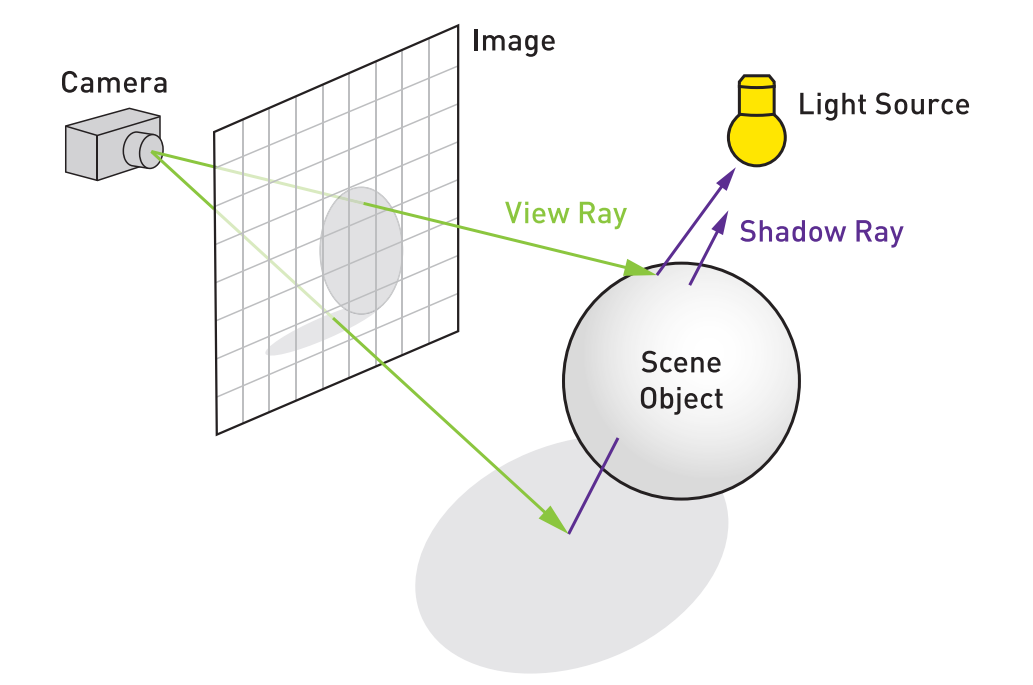
\includegraphics[width=12.0cm]{Fig1-1.png}
	\caption{光线投射。一束光线从摄像机的位置出发穿过像素网格进入场景中。在每个位置,朝光源投射另一束光线来决定表面被照亮还是在阴影里。(图片来源 Henrik,“光线追踪(图形学)”, 维基百科)}
	\label{Fig1-1}
\end{figure*}
 
\textit{光线追踪}利用光线投射机制来递归的采集反射和折射物体对光的贡献。比如,当光线碰到一个镜子,从镜子上的碰撞点投射一束光到反射方向。不管这个反射光线和什么相交都会影响镜子最终的渲染。同样的,透明或者玻璃物体可能会同时产生反射光和折射光。这个过程会递归的发生,新的光线也可能会产生新的反射光线和折射光线。递归通常都会有截止限制,比如光线最大反弹次数。整个光线树会被反向的沿着光路评估,最后计算出颜色。和之前一样,我们会查询每个碰撞点,在碰撞点向每个光源发射光线来决定它是否在阴影里。见图\ref{Fig1-2}。

\begin{figure*}
	\centering
	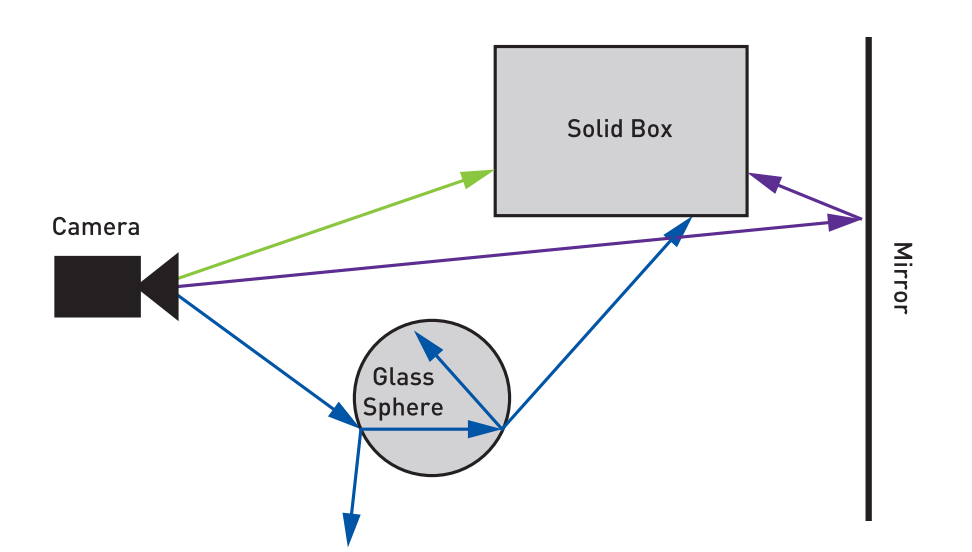
\includegraphics[width=12.0cm]{Fig1-2.png}
	\caption{光线追踪。三束光线从摄像机射入场景。最上方绿色的光线直接击中盒子。中间紫色的光线先击中镜子,经反射击中盒子的背部。最下方蓝色光线击中玻璃球,产生反射和折射光线。折射光线接着产生两个子光线,其中一束穿过玻璃球的光线又产生两束光线。}
	\label{Fig1-2}
\end{figure*}


在Whitted的方法(传统的光线追踪方法)中,他们假设物体表面绝对闪亮和光滑,光源是方向光源或者在无穷远处。 在Cook的方法(\textit{随机光线追踪}法)中,光线树中每个节点可以发射更多的光线以产生各种效果。比如一个球形光源而不是一个点光源,可以照亮局部的物体表面,所以我们可以射出很多光线到球上不同的位置来估计有多少光照到达。 当我们对可见的面光源进行积分,完全在阴影里的点落在\textit{全影}区域,局部光照点落在\textit{半影}区域。见图\ref{Fig1-3}。

\begin{figure*}
	\centering
	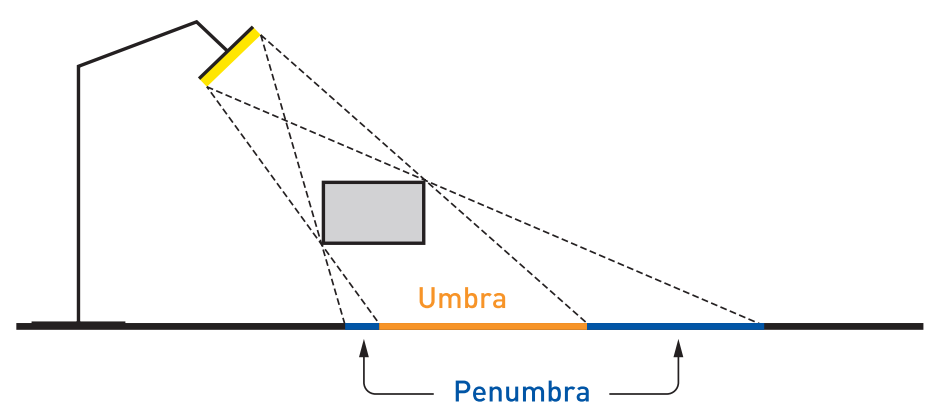
\includegraphics[width=12.0cm]{Fig1-3.png}
	\caption{面光源投射出柔和半影区域,全影区域完全在阴影当中。}
	\label{Fig1-3}
\end{figure*}


通过向反射方向上的锥形区域射出很多光线并对结果进行混合,我们可以得到有光泽的反射而不是镜面反射。见图\ref{Fig1-4}。这种分散采样的方法同样可以用来对半透明,景深,运动模糊等效果建模。

\begin{figure*}
	\centering
	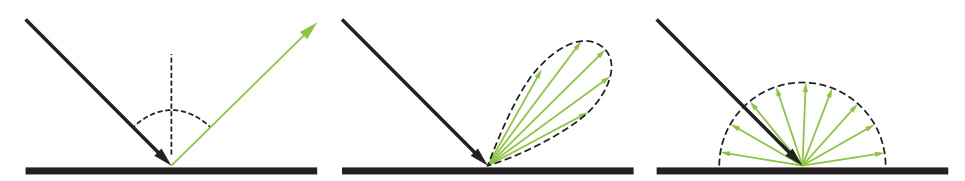
\includegraphics[width=12.0cm]{Fig1-4.png}
	\caption{镜面反射,光泽反射,漫反射。左侧:入射光线被反射后朝一个方向离开镜面。中间:表面被打磨过,比如黄铜,在反射方向附近反射光线并使的表面有光泽。右边:材料是漫反射或哑光的,比如石膏,入射光线朝所有的方向反射。}
	\label{Fig1-4}
\end{figure*}

在真实世界当中有很多光源发射光线,他们到达人的眼睛的方法多种多样,包括折射和反射。\textit{光泽}表面反射光线到很多方向上,不仅仅是在反射方向上。\textit{漫反射}或者\textit{哑光}表面可以将光线分散到更广泛的范围。在光线追踪领域,我们反转了光的散射行为,我们使用出射方向和材料来帮助我们决定各个入射方向上光线对物体表面渲染的重要性。

跟踪如此复杂的光线传输很快就变得令人不能承受,也很容易造成低效的渲染。为了产生一张图像,我们只需要光线从一些特定的方向穿过摄像机的镜头。 \textit{递归光线追踪}法在很多方面反转了光线传播的物理过程,按照将会影响图像的方向从人眼处产生光线。

在Kajiya风格或路径跟踪中,光线反射到场景中的哑光表面上,它允许现实世界中的所有光路(除了相位效果比如衍射)。 这里的光路指的是一系列光 - 物体相互作用,它们从相机开始并在一个光源处结束。

结合表面的反射属性,我们需要在每个表面交叉点的位置估算它周围所有光线的贡献。例如,一堵红色的墙旁边有白色的屋顶,墙会发射红色的光到屋顶,反之亦然。 墙和屋顶会产生进一步的相互反射,因为他们之间会进一步互相反射反射光线,这也会影响到彼此。从眼睛的视角递归的叠加这些效果,当碰到光源的时候结束,一个真正的基于物理的图像就\textit{可能}生成了。

这里我们使用了“可能”,如果我们在一个粗糙的表面射出一组光,比方说一千束。然后对于每一束光,我们递归的发射出另外上千条,持续不停直到碰到光源,那我们光是计算一个像素点就可以到天荒地老了。相反,当一束光线从人眼发射出去并碰到一个可见的表面上,在碰撞点光线追踪器在有用的方向上只产生一束光。这束光依次产生一束光并持续下去,这些光线并最终形成一个路径。对于一个像素,将多个追踪的路径进行混合就可以估计出像素真正的辐射。当计算更多的路径时,最后的效果也会提升。通过适当的处理,路径追踪可以给出\textit{无偏}的结果,这个结果符合物理真实。

大多数现代光线追踪器每个像素使用不止一束光线作为蒙特卡洛(MC)算法的底层部分。Cook风格和Kajiya风格的算法就是例子。这些方法都有对空间中各种概率密度函数(PDFs)的理解。比如,在Cook风格算法中,我们可能会在一个透镜区域包含一个PDF。在基于路径的方法中,PDF将会在我们称为\textit{路径空间}的路径上出现。

为了减少误差,令蒙特卡洛算法的PDF采样不均匀称为\textit{重要性采样}。使用数论方法中的样本低差异模式而不是传统的伪随机数生成器来创建随机样本被称为拟蒙特卡罗(QMC)采样。在很大程度上,计算机图形学从业者使用MC和QMC领域的标准术语。然而,这种做法会造成同义词混淆。比如,计算机图形学中的“阴影光线直接照明”(direct illumination with shadow rays)是MC/QMC领域中“下一事件估计”(next event estimation)的一个例子。

从形式化的角度,渲染器就是求解一个针对图形学特定问题的传播方程,也经常被称作\textit{渲染方程}。 这个方程经常写做表面上一点处的能量平衡方程。在一些文献中符号会有变化,但是都和下面的公式很相似:

\begin{equation}
L_o(P, \omega_o) = \int_{s^2} f(P, \omega_o,\omega_i)L_i(P,\omega_i) |cos\theta_i|d\omega_i
\end{equation}

这里,$L_o$是在$\omega_o$方向离开表面点$P$的辐射,表面属性$f$是双向反射分布函数(BRDF)。这个函数也经常标记为$f_r$或者$\rho$。 $L_i$ 是$\omega_i$方向上的入射光线,表面法线和入射光线的夹角是$\theta_i$, $|cos \theta_i|$表示这个角度的几何衰减。通过积分所有表面和物体光的效果,不仅仅是光源,和所有入射方向,折叠表面BRDF效果,我们得出辐射,实质上就是光线的颜色。因为$L_i$通常是递归计算的,比如从点$P$所有可见的表面都要依次计算得到辐射值,使用路径追踪和相关方法选择他们当中所有可能的路径,选择的目标是沿着路径方向投射每条光线,这个方向对于计算所有可能方向效果的良好近似很重要。

通常点$P$会被隐式的略去。而且,波长$\lambda$可以作为函数的输入。也有包含\textit{参与媒介}的更泛化的方程,比如烟,雾和物理光学效应比如衍射。

关于\textit{参与媒介},\textit{ray marching} 是在一个区间里沿着光线前进并在光线方向采样的过程。这种投射光线的方法经常用来做体积渲染,在这种场景里没有特定的表面。除此之外,可以通过一些方法来计算光线在体积内每个位置的效果。ray marching还可以用来仿真体积内的碰撞。

通常在 Hart球面追踪算法\cite{Hart1996}的一些变体下,ray marching 经常被用来求解和隐式距离方程定义的曲面的交叉或者沿光线到表面的方向采样和搜索来进行体内/体外测试。这里的“球面”是距离物体表面等距离的点形成的球。它和交叉球无关。按照之前的表示方法,这个过程应该称为“球体投射”而不是“球体追踪”。这种类型的求交检测经常在示例场景出现,并因Shadertoy网站而在网络上变得流行。

我们只接触到光线相关渲染技术的基础部分和使用的术语。更多有关资源的指南,请参阅本书的网站:http://raytracinggems.com。
 
\bibliographystyle{unsrt}
\bibliography{ref}
\end{document}




